\documentclass{scrreprt}

\usepackage{aligned-overset}
\usepackage{amsmath}
\usepackage{amssymb}
\usepackage{bm}
\usepackage[shortlabels]{enumitem}
\usepackage{hyperref}
\usepackage[utf8]{inputenc}
\usepackage{multicol}
\usepackage{mathtools}
\usepackage{physics}
\usepackage{tabularx}
\usepackage[table]{xcolor}
\usepackage{titling}
\usepackage{fancyhdr}
\usepackage{xfrac}
\usepackage{pgfplots}

\pgfplotsset{compat = newest}
\usetikzlibrary{intersections}
\usetikzlibrary{patterns}
\usepgfplotslibrary{fillbetween}

\author{Karsten Lehmann}
\date{WiSe 2021/2022}
\title{Übungsblatt 02\\Lineare Algebra - Grundlegende Konzepte}

\setlength{\headheight}{26pt}
\pagestyle{fancy}
\fancyhf{}
\lhead{\thetitle}
\rhead{\theauthor}
\lfoot{\thedate}
\rfoot{Seite \thepage}

\newcommand\ccg[1]{\cellcolor{green}{#1}}

\begin{document}
\paragraph{Aufgabe 2} Gegeben ist das gleichseitige Dreieck:

\begin{tikzpicture}
  \node[below left] at (0, 0) {A};
  \node[below right] at (3, 0) {B};
  \node[above] at (1.5, 2.598) {C};
  \draw[thick] (0, 0) -- (3, 0) -- (1.5, 2.598) -- cycle;
\end{tikzpicture} \\
Die Drehung des gegebenen Dreiecks gegen den Uhrzeigersinn um den Mittelpunkt
um $120^{\circ}$ (bzw. um $240^{\circ}$, bzw. um $360^{\circ}$) bezeichnen wir
mit $r_1$ (bzw. mit $r_2$, bzw. mit id). \\
Die Spiegelung des Dreiecks an den Höhen durch die Eckpunkte $A$, $B$ und $C$
werden mit $s_1$, $s_2$ und $s_3$ bezeichnet.

Man kann alle genannten Drehungen und Spiegelungen als Abbildungen auffassen -
somit kann man auch Kompositionen dieser betrachten. \\
Sei $D_6 \coloneqq \qty\big{\text{id}, r_1, r_2, r_3, s_1, s_2, s_3}$.

\begin{enumerate}[(1)]
\item \label{sec:2_1}
  Zeigen Sie, dass $D_6$ mit der Komposition von Abbildungen $\circ$ eine
  nicht-abelsche Gruppe ist.
  Stellen Sie die Gruppe $\qty\big(D_6, \circ)$ mithilfe einer
  Multiplikationstafel dar.

  \subparagraph{Lsg.} \underline{Multiplikationstabelle:} \\
  \begin{tabular}{c|>{\columncolor{yellow}}cccccc}
    $\circ$             & id       & $r_1$    & $r_2$       & $s_1$       & $s_2$       & $s_3$ \\
    \hline
    \rowcolor{yellow}id & \ccg{id} & $r_1$    & $r_2$       & $s_1$       & $s_2$       & $s_3$ \\
    $r_1$               & $r_1$    & $r_2$    & \ccg{id}    & $s_3$       & $s_1$       & $s_2$ \\
    $r_2$               & $r_2$    & \ccg{id} & $r_1$       & $s_2$       & $s_3$       & $s_1$ \\
    $s_1$               & $s_1$    & $s_3$    & $s_2$       & \ccg{id}    & $r_1$       & $r_2$ \\
    $s_2$               & $s_2$    & $s_1$    & $s_3$       & $r_2$       & \ccg{id}    & $r_1$ \\
    $s_3$               & $s_3$    & $s_2$    & $s_1$       & $r_1$       & $r_2$       & \ccg{id} \\
  \end{tabular} \\
  Nun heißt $\qty\big(D_6, \circ)$ eine Gruppe, falls
  \begin{enumerate}[(i)]
  \item Für $a, b, c \in D_6$ gilt
   $\qty\big(a \circ b) \circ c = a \circ \qty\big(b \circ c)$
    (\emph{Assoziativität}).
  \item ein \emph{neutrales Element} $e \in D_6$ existiert, sodass für jedes
    $a \in D_6$ gilt $e \circ a = a \circ e = a$.
    Das neutrale Element in $D_6$ ist \colorbox{yellow}{``id''}.
  \item für jedes Element $a \in D_6$ ein \emph{inverses Element}
    $a^{-1} \in D_6$ existiert mit \\
    \colorbox{green}{$a \circ a^{-1} = e =$ id}.
  \end{enumerate}

  \newpage
  Die Gruppe $\qty\big(D_6, \circ)$ heißt zusätzlich eine kommutative oder
  abelsche Gruppe, falls für $a, b \in D_6$ gilt $a \circ b = b \circ a$.
  Sei nun $a = s_2$ und $b = s_3$.
  Dann ergibt $b \circ a$:

  \begin{tikzpicture}
    \node[below left] at (0, 0) {A};
    \node[below right] at (1, 0) {B};
    \node[above] at (0.5, 0.866) {C};
    \draw[thick] (0, 0) -- (1, 0) -- (0.5, 0.866) -- cycle;
    \draw[black!60!green] (-0.5, 1) -- (1, 0);

    \node at (2.5, 0.4) {$\overset{{\color{black!60!green}\text{Spiegelung an $s_2$}}}\Rightarrow$};

    \node[below left] at (4, 0) {C};
    \node[below right] at (5, 0) {B};
    \node[above] at (4.5, 0.866) {A};
    \draw[thick] (4, 0) -- (5, 0) -- (4.5, 0.866) -- cycle;
    \draw[blue] (4.5, 0.866) -- (4.5, -0.866);

    \node at (6.5, 0.4) {$\overset{{\color{blue}\text{Spiegelung an $s_3$}}}\Rightarrow$};

    \node[below left] at (8, 0) {B};
    \node[below right] at (9, 0) {C};
    \node[above] at (8.5, 0.866) {A};
    \draw[thick] (8, 0) -- (9, 0) -- (8.5, 0.866) -- cycle;
  \end{tikzpicture} \\
  und $a \circ b$: \\
  \begin{tikzpicture}
    \node[below left] at (0, 0) {A};
    \node[below right] at (1, 0) {B};
    \node[above] at (0.5, 0.866) {C};
    \draw[thick] (0, 0) -- (1, 0) -- (0.5, 0.866) -- cycle;
    \draw[blue] (0.5, 0.866) -- (0.5, -0.866);

    \node at (2.5, 0.4) {$\overset{{\color{blue}\text{Spiegelung an $s_3$}}}\Rightarrow$};

    \node[below left] at (4, 0) {B};
    \node[below right] at (5, 0) {A};
    \node[above] at (4.5, 0.866) {C};
    \draw[thick] (4, 0) -- (5, 0) -- (4.5, 0.866) -- cycle;
    \draw[black!60!green] (3.5, 1) -- (5, 0);

    \node at (6.5, 0.4) {$\overset{{\color{black!60!green}\text{Spiegelung an $s_2$}}}\Rightarrow$};

    \node[below left] at (8, 0) {C};
    \node[below right] at (9, 0) {A};
    \node[above] at (8.5, 0.866) {B};
    \draw[thick] (8, 0) -- (9, 0) -- (8.5, 0.866) -- cycle;
  \end{tikzpicture} \\
  $\Rightarrow a \circ b \ne b \circ a$ \\
  $\Rightarrow \qty\big(D_6, \circ)$ ist eine nicht-abelsche Gruppe.

\item Geben Sie das neutrale Element von der Gruppe $\qty\big(D_6, \circ)$ an.

  \subparagraph{Lsg,} Wie in der Multiplikationstafel in \hyperref[sec:2_1]{(1)}
  zu sehen ist \colorbox{yellow}{id} das neutrale Element der Gruppe, da für
  alle $a \in D_6$ gilt $a \circ \text{id} = \text{id} \circ a = a$.

\item Geben Sie für jedes Element von $D_6$ sein Inverses an.

  \subparagraph{Lsg.} Wie in der Multiplikationstafel in \hyperref[sec:2_1]{(1)}
  \colorbox{green!40}{hervorgehoben:}
  \begin{multicols}{2}
    \begin{itemize}
    \item $\text{id} \circ \text{id} = \text{id}$
    \item $r_1 \circ r_2 = \text{id}$
    \item $r_2 \circ r_1 = \text{id}$
    \item $s_1 \circ s_1 = \text{id}$
    \item $s_2 \circ s_3 = \text{id}$
    \item $s_2 \circ s_3 = \text{id}$
    \end{itemize}
  \end{multicols}

\item Zeigen Sie, dass $\qty\big{\text{id}, r_1, r_2}$ eine Untergruppe von
  $D_6$ ist.

  \subparagraph{Lsg.} Die Teilmenge $\qty\big{\text{id}, r_1, r_2} \subset D_6$
  wird Untergruppe von $D_6$ genannt, falls
  \begin{enumerate}[1)]
  \item $1_{D_6} \in \qty\big{\text{id}, r_1, r_2}$
    $\Rightarrow$ Das neutrale Element ``id'' ist in
    $\qty\big{\text{id}, r_1, r_2}$ enthalten.

  \item Für $a, b \in \qty\big{\text{id}, r_1, r_2}$ gilt
    $a \circ b \in \qty\big{\text{id}, r_1, r_2}$

     \begin{multicols}{3}
       \begin{itemize}
       \item $\text{id} \circ \text{id} = \text{id}$
       \item $\text{id} \circ r_1 = r_1$
       \item $\text{id} \circ r_2 = r_2$
       \item $r_1 \circ \text{id} = r_1$
       \item $r_1 \circ r_1 = r_2$
       \item $r_1 \circ r_2 = \text{id}$
       \item $r_2 \circ \text{id} = r_2$
       \item $r_2 \circ r_1 = \text{id}$
       \item $r_2 \circ r_2 = r_1$
       \end{itemize}
     \end{multicols}
  \item Für $a \in \qty\big{\text{id}, r_1, r_2}$ gilt
    $a^{-1} \in \qty\big{\text{id}, r_1, r_2}$. \\
    Es existiert für jedes Element ein Inverses, nämlich
    ``id'' für ``id'', $r_2$ für $r_1$ und $r_1$ für $r_2$.
  \end{enumerate}
\end{enumerate}

\paragraph{Aufgabe 5} Sei $K \coloneqq \mathbb{R} \times \mathbb{R}$.
\begin{enumerate}[(1)]
\item \label{sec:5_1}
  Für $\qty\big(a, b), \qty\big(a', b') \in K$ sei
  \[
    \qty\big(a, b) + \qty\big(a', b') \coloneqq \qty\big(a + a', b + b')
  \]
  \[
    \qty\big(a, b) \circ \qty\big(a', b') \coloneqq
    \qty\big(aa' - bb', ab' + a'b)
  \]
  Zeigen Sie, dass $\qty\big(K, +, \circ)$ ein Körper ist.

  \subparagraph{Lsg.} Für $\qty\big(K, +)$ gilt
  \begin{enumerate}[(i)]
  \item Für $\qty\big(a, a'), \qty\big(b, b'), \qty\big(c, c') \in K$ ist
    \begin{flalign*}
      \qty\big(a, a') + \qty\Big(\qty\big(b, b') + \qty\big(c, c'))
      &= \qty\big(a, a') + \qty\big(b + c, b' + c') & \\
      &= \qty\big(a + b + c, a' + b' + c') \\
      &= \qty\Big(\qty\big(a + b, a' + b')) + \qty\big(c, c') \\
      &= \qty\Big(\qty\big(a, a') + \qty\big(b, b')) + \qty\big(c, c')
    \end{flalign*}
    $\Rightarrow \qty\big(K, +)$ ist assoziativ.

  \item Für jedes $\qty\big(a, a') \in K$ gilt
    \[
      \qty\big(a, a') + \qty\big(0, 0)
      = \qty\big(a + 0, a' + 0) = \qty\big(a, a')
      = \qty\big(0 + a, 0 + a')
      = \qty\big(0, 0) + \qty\big(a, a')
    \]
    $\Rightarrow \qty\big(0, 0)$ ist neutrales Element von $\qty\big(K, +)$

  \item Seien $a, a' \in \mathbb{R}$ beliebig.
    Da $\mathbb{R}$ ein Körper ist, existieren $-a, -a' \in \mathbb{R}$
    mit $a + (-a) = 0$ und $a' + \qty\big(-a') = 0$.
    Somit existiert für jedes $\qty\big(a, a') \in K$ auch
    $\qty\big(-a, -a') \in K$ mit
    $\qty\big(a, a') + \qty\big(-a, -a') = \qty\big(0, 0)$.
  \end{enumerate}

  $\Rightarrow \qty\big(K, +)$ ist eine \textbf{Gruppe}.

  Weiterhin ist für $\qty\big(a, a'), \qty\big(b, b') \in K$
  \begin{flalign*}
    \qty\big(a, a') + \qty\big(b, b') &= \qty\big(a + b, a' + b') & \\
    \overset{\text{Kommutativität in $\mathbb{R}$}}&= \qty\big(b + a, b' + a') \\
    &= \qty\big(b, b') + \qty\big(a, a')
  \end{flalign*}
  $\Rightarrow \qty\big(K, +)$ ist eine \textbf{abelsche Gruppe}.

  Für $\qty\big(K, +, \circ)$ gilt
  \begin{enumerate}[(i)]
  \item $\qty\big(K, +)$ ist eine abelsche Gruppe (siehe oben).
  \item Für $\qty\big(a, a'), \qty\big(b, b'), \qty\big(c, c') \in K$ gilt:
    \begin{flalign*}
      \qty\Big(\qty\big(a, a') \circ \qty\big(b, b')) \circ \qty\big(c, c')
      &= \qty\big(ab - a'b', ab' + ba') \circ \qty\big(c, c') & \\
      &= \qty\Big(
        \qty\big(ab - a'b') \cdot c - \qty\big(ab' + ba') \cdot c',
        \qty\big(ab - a'b') \cdot c' + \qty\big(ab' + ba') \cdot c
      ) \\
      &= \qty\Big(
        abc - a'b'c - ab'c' - ba'c',
        abc' - a'b'c' + ab'c + ba'c
      ) \\
      &= \qty\Big(
        a \cdot \qty\big(bc - b'c') - a' \cdot \qty\big(b'c + bc'),
        a \cdot \qty\big(bc' + b'c) + a' \cdot \qty\big(bc - b'c')
      ) \\
      &= \qty\big(a, a') \circ \qty\big(bc - b'c', bc' + cb') \\
      &= \qty\big(a, a') \circ \qty\Big(\qty\big(b, b') \circ \qty\big(c, c'))
    \end{flalign*}

    $\Rightarrow \qty\big(K, +, \circ)$ ist assoziativ bezüglich der
    Multiplikation.

  \item Sei $1_K = \qty\big(1, 0)$.
    Dann ist $1_k \ne 0_K = \qty\big(0, 0)$.
    Weiterhin gilt für jedes Element $\qty\big(a, a') \in K$:
    \begin{flalign*}
      \qty\big(a, a') \circ \qty\big(1, 0)
      &= \qty\big(a \cdot 1 - a' \cdot 0, a \cdot 0 + 1 \cdot a') \\
      &= \qty\big(a, a') \\
      &= \qty\big(1 \cdot a - 0 \cdot a', 1 \cdot a' + a \cdot 0) \\
      &= \qty\big(1, 0) \circ \qty\big(a, a')
    \end{flalign*}
    $\Rightarrow \qty\big(K, +, \circ)$ besitzt mit $\qty\big(1, 0)$ ein
    neutrales Element der Multiplikation.

  \item Seien $\qty\big(a, a'), \qty\big(b, b'), \qty\big(c, c') \in K$
    beliebig, dann
    \begin{flalign*}
      \qty\big(a, a') \circ \qty\Big(\qty\big(b, b') + \qty\big(c, c'))
      &= \qty\big(a, a') \circ \qty\big(b + c, b' + c') \\
      &= \qty\Big(
        a \cdot \qty\big(b + c) - a' \cdot \qty\big(b' + c'),
        a \cdot \qty\big(b' + c') + a' \cdot \qty\big(b + c)
      ) \\
      &= \qty\big(ab + ac - a'b' - a'c', ab' + ac' + a'b + a'c) \\
      &= \qty\big(ab - a'b', ab' + a'b) + \qty\big(ac - a'c', ac' + a'c) \\
      &= \qty\big(a, a') \circ \qty\big(b, b') +
        \qty\big(a, a') \circ \qty\big(c, c')
    \end{flalign*}
    und
    \begin{flalign*}
      \qty\Big(\qty\big(b, b') + \qty\big(c, c')) \circ \qty\big(a, a')
      &= \qty\big(b + c, b' + c') \circ \qty\big(a, a') \\
      &= \qty\Big(
        \qty\big(b + c) \cdot a - \qty\big(b' + c') \cdot a',
        \qty\big(b + c) \cdot a' + a \cdot \qty\big(b' + c')
      ) \\
      &= \qty\big(
        ba + ca - b'a' - c'a',
        ba' +ca' + ab' + ac'
      ) \\
      &= \qty\big(ba - b'a', ba' + ab') + \qty\big(ca - c'a', ca' + ac') \\
      &= \qty\big(b, b') \circ \qty\big(a, a') +
        \qty\big(c, c') \circ \qty\big(a, a')
    \end{flalign*}
    $\Rightarrow \qty\big(K, +, \circ)$ ist distributiv.
  \end{enumerate}
  $\Rightarrow \qty\big(K, +, \circ)$ ist ein \textbf{Ring}.
  \newpage
  Außerdem gilt für $\qty\big(a, a'), \qty\big(b, b') \in K$ noch
  \begin{flalign*}
    \qty\big(a, a') \cdot \qty\big(b, b')
    &= \qty\big(ab - a'b', ab' + ba') \\
    \overset{\text{Kommutativität in $\mathbb{R}$}}&=
    \qty\big(ba - b'a', ba' + ab') \\
    &= \qty\big(b, b') \circ \qty\big(a, a')
  \end{flalign*}
  $\Rightarrow \qty\big(K, +, \circ)$ ist assoziativ bezüglich der
  Multiplikation. \\

  Sei nun $\qty\big(a, a') \ne \qty\big(0, 0) \in K$ beliebig.
  Dann ist
  $\qty(\frac{a}{a^2 + \qty(a')^2}, -\frac{a'}{a^2 + \qty(a')^2}) \in K$.
  \begin{flalign*}
    \qty\big(a, a') \circ
      \qty(\frac{a}{a^2 + \qty(a')^2}, -\frac{a'}{a^2 + \qty(a')^2})
    &= \qty(
      a \cdot \frac{a}{a^2 + \qty(a')^2} - a' \cdot \frac{-a'}{a^2 + \qty(a')^2},
      a \cdot \frac{-a'}{a^2 + \qty(a')^2} + \frac{a}{a^2 + \qty(a')^2} \cdot a'
      ) \\
    &= \qty(
      \frac{a^2}{a^2 + \qty(a')^2} - \frac{\qty(a')^2}{a^2 + \qty(a')^2},
      \frac{aa'}{a^2 + \qty(a')^2} - \frac{a'a}{a^2 + \qty(a')^2}
    ) \\
    &= \qty(
      \frac{a^2 + \qty(a')^2}{a^2 + \qty(a')^2},
      \frac{0}{a^2 + \qty(a')^2}
    ) \\
    &= \qty\big(1, 0)
  \end{flalign*}
  $\Rightarrow$ für jedes Element $a \ne 0 \in K$ existiert ein multiplikatives
  Inverses. \\
  $\Rightarrow \qty\big(K, +, \circ)$ ist ein \textbf{Körper}.

\item Was ist $i^2$?

  \subparagraph{Lsg.} $i = \qty\big(0, 1)$.
  Somit ist $i^2 = i \circ i =
  \qty\big(0 \cdot 0 - 1 \cdot 1, 1 \cdot 0 + 0 \cdot 1) = \qty\big(-1, 0)$.


\item Definieren Sie nun $\qty\big(a, b) \cdot \qty\big(a', b') =
  \qty\big(aa', bb')$.
  Beweisen Sie, dass $\qty\big(K, +, \cdot)$ ein Ring ist.
  Handelt es sich um einen Körper?
  Handelt es sich um einen Integritätsring?

  \subparagraph{Lsg.} Aus \hyperref[sec:5_1]{(1)} ist bereits bekannt, dass
  $\qty\big(K, +)$ eine abelsche Gruppe ist.
  Weiter gilt für $\qty\big(a, a'), \qty\big(b, b'), \qty\big(c, c') \in K$:
  \begin{flalign*}
    \qty\Big(\qty\big(a, a') \cdot \qty\big(b, b')) \cdot \qty\big(c, c')
    &= \qty\big(ab, a'b') \cdot \qty\big(c, c') \\
    &= \qty\big(abc, a'b'c') \\
    &= \qty\big(a, a') \cdot \qty\big(bc, b'c') \\
    &= \qty\big(a, a') \cdot \qty\Big(\qty\big(b, b') \cdot \qty\big(c, c'))
  \end{flalign*}
  $\Rightarrow \qty\big(K, +, \cdot)$ ist assoziativ bezüglich der
  Multiplikation.

  Zusätzlich ist $\qty\big(1, 1) \in K$.
  Es gilt für $\qty\big(a, a') \in K$:
  \[
    \qty\big(a, a') \cdot \qty\big(1, 1)
    = \qty\big(a \cdot 1, a' \cdot 1)
    = \qty\big(a, a')
    = \qty\big(1 \cdot a, 1 \cdot a')
    = \qty\big(1, 1) \cdot \qty\big(a, a')
  \]
  $\Rightarrow \qty\big(1, 1)$ ist neutrales Element der Multiplikation.

  \newpage
  Für $\qty\big(a, a'), \qty\big(b, b'), \qty\big(c, c') \in K$ gilt:
  \begin{flalign*}
    \qty\big(a, a') \cdot \qty\Big(\qty\big(b, b') + \qty\big(c, c'))
    &= \qty\big(a, a') \cdot \qty\big(b + c, b' + c') \\
    &= \qty\Big(a \cdot \qty\big(b + c), a' \cdot \qty\big(b' + c')) \\
    \overset{\text{Distributivität in $\mathbb{R}$}}&=
      \qty\big(ab + ac, a'b' + a'c') \\
    &= \qty\big(ab, a'b') + \qty\big(ac, a'c') \\
    &= \qty\big(a, a') \cdot \qty\big(b, b')
      + \qty\big(a, a') \cdot \qty\big(c, c')
  \end{flalign*}
  und
  \begin{flalign*}
    \qty\Big(\qty\big(b, b') + \qty\big(c, c')) \cdot \qty\big(a, a')
    &= \qty\big(b + c, b' + c') \cdot \qty\big(a, a') \\
    &= \qty\Big(\qty\big(b + c) \cdot a, \qty\big(b' + c') \cdot a') \\
    \overset{\text{Distributivität in $\mathbb{R}$}}&=
      \qty\big(ba + ca, b'a' + c'a') \\
    &= \qty\big(ba, b'a') + \qty\big(ca, c'a') \\
    &= \qty\big(b, b') \cdot \qty\big(a, a') +
      \qty\big(c, c') \cdot \qty\big(a, a')
  \end{flalign*}
  $\Rightarrow \qty\big(K, +, \cdot)$ ist distributiv.

  $\Rightarrow \qty\big(K, +, \cdot)$ ist ein \textbf{Ring}.

  Für $\qty\big(a, a'), \qty\big(b, b') \in K$ gilt
  \[
    \qty\big(a, a') \cdot \qty\big(b, b')
    = \qty\big(ab, a'b')
    \overset{\text{Kommutativität in $\mathbb{R}$}}= \qty\big(ba, b'a')
    = \qty\big(b, b') \cdot \qty\big(a, a')
  \]
  $\Rightarrow \qty\big(K, +, \cdot)$ ist ein \textbf{kommutativer Ring}. \\

  Sei nun $\qty\big(a, 0) \ne \qty\big(0, 0) \in K$ beliebig.
  Angenommen es gäbe ein inverses Element $\qty\big(b, b') \in K$, dann
  würde gelten
  \[
    \qty\big(a, 0) \cdot \qty\big(b, b') = \qty\big(1, 1)
  \]
  Ein solches Element kann nicht existieren, da kein $b'$ mit
  $0 \cdot b' = 1$ existiert.

  $\Rightarrow$ nicht jedes Element verschieden von $\qty\big(0, 0)$ in
  $\qty\big(K, +, \cdot)$ ist invertierbar.

  $\Rightarrow \qty\big(K, +, \cdot)$ ist \textbf{kein Körper}. \\

  Offensichtlich sind $\qty\big(1, 0) \ne \qty\big(0, 0) \in K$
  und $\qty\big(0, 1) \ne \qty\big(0, 0) \in K$.
  Der Ring $\qty\big(K, +, \cdot)$ heißt Integritätsring, falls
  \[
    a \cdot b = 0 \Rightarrow a = 0 \lor b = 0
  \]

  Nun ist $\qty\big(1, 0) \cdot \qty\big(0, 1) = \qty\big(1 \cdot 0, 0 \cdot 1)
  = \qty\big(0, 0)$ ein Widerspruch.

  $\Rightarrow \qty\big(K, +, \cdot)$ ist kein Integritätsring.
\end{enumerate}
\end{document}